%\documentclass[journal]{jasse-modern}
%\documentclass[proceedings,links]{jasse-modern}% Enable clickable links.
\documentclass[proceedings]{jasse-modern}% Switch the active mode here.
%
%%%%%%%%%%%%%%%%%%%
% Article information
%%%%%%%%%%%%%%%%%%%
\JasseSetup{
  year = {20xx},
  vol = {xx},
  number = {x},
  pages = {xx--xx},
  received = {xx},
  accepted = {xx},
  published = {xx},
}

%
%%%%%%%%%%%%%%%%%%%
% If you use another package or new command,
% please add as below.
%%%%%%%%%%%%%%%%%%%
%\usepackage{color}
%\usepackage{hyperref}
\usepackage{siunitx}
\newcommand{\A}{\mathcal{A}}
\newcommand{\mcc}[1]{\multicolumn{1}{c}{#1}}
\sisetup{
  detect-all,
  exponent-product = \times,
}
%%%%%%%%%%%%%%%%%%%
%
%
%%%%%%%%%%%%%%%%%%%
% Title is here.
%%%%%%%%%%%%%%%%%%%
\title{Template of JSST2026 (ver.1.0)\\ Instructions for preparing your manuscript}

%%%%%%%%%%%%%%%%%%%
% Author is listed below.
%%%%%%%%%%%%%%%%%%%
\author[1,*]{Alfred Author}% Corresponding author should add * mark.
\author[2,4]{Benjamin Author}
\author[3]{Charles Author}

%%%%%%%%%%%%%%%%%%%
% Affiliation
%%%%%%%%%%%%%%%%%%%
\affil[1]{{Department of Simulation, School of Technology, Japan University}}
\affil[2]{{Affiliation 2}}
\affil[3]{{Affiliation 3}}
\affil[4]{{Affiliation 4}}

%%%%%%%%%%%%%%%%%%%
% Date must be empty.
%%%%%%%%%%%%%%%%%%%
%\dates{\today}

%%%%%%%%%%%%%%%%%%%
% Put email address
%%%%%%%%%%%%%%%%%%%
\email{mail@mail.edu}% Corresponding author's address

\begin{document}
\maketitle
\thispagestyle{titlepage}

%%%%%%%%%%%%%%%%%%%
% Abstract
%%%%%%%%%%%%%%%%%%%
\begin{abstract}
This is a {\LaTeX} template/instructions for The 45th International Conference on Simulation Technology (JSST2026).
This version of the template was prepared on \today.
The authors must provide the paper title, authors' name, affiliation, and corresponding author's email address.
Abstract is written here.
Moreover, the authors must provide keywords below.
It is essential to adhere to this template because your manuscripts are printed as
submitted with minimal editing/formatting by publisher.
Do not modify any formats or styles.
Visit \url{http://jsst-conf.jp/2026/} for the latest version of JSST2026 template.
\end{abstract}

%%%%%%%%%%%%%%%%%%%
% Keywords
%%%%%%%%%%%%%%%%%%%
\begin{keywords}
Computer simulation, Numerical methods
\end{keywords}

%%%%%%%%%%%%%%%%%%%
% Start main body
%%%%%%%%%%%%%%%%%%%
\section{Introduction}

This template provides formatting guidelines for JSST2026 proceedings papers. It is essential to adhere to this template because your manuscript will be published ``as is'' with minimal copy-editing. Do not modify formats (font, font size, paper size, printing area, line spacing, etc.). Authors should prepare manuscripts using the official formats (LaTeX or Word style), in which all styles and formats are prescribed. Use this file as a template. Manuscripts for JSST2026 must be submitted electronically only.

\section{Paper length}
Authors should prepare their manuscripts according to the guidelines on the web page:
\begin{center}
\url{http://jsst-conf.jp/2026/}
\end{center}
The LaTeX style file and MS Word template file can be downloaded from this page.
The minimum acceptable length of the manuscript is 4 pages of an A4-sized PDF file.

\section{Typographical style}
\subsection{Equations}
Equations are centered with the equation number (in Arabic) appearing in the right-hand margin, in
parentheses:
\begin{align}\label{eqn:1}
  \left\{
  \begin{alignedat}{2}
    i\frac{\partial u}{\partial t}-\Delta u+\kappa|u|^2u &= 0
      &\qquad& \text{in } \Omega\times[0,\infty),\\[2mm]
    u(x,t) &= 0
      && \text{in } \Gamma\times[0,\infty),\\[2mm]
    u(x,0) &= u_0(x).
  \end{alignedat}
  \right.
\end{align}
Long equations can be split across multiple lines but avoid leading to misinterpretation.
Equations are referenced in the main text as \eqref{eqn:1}.

\subsection{Theorem, Algorithm, etc.}
Examples of theorem-style environments are as follows:
%Theorem style is already included in jasse-modern.cls.
%The following are examples:

\begin{theorem}[Newton's apple]
This is a theorem style of template on JSST2026 proceedings papers.
\end{theorem}

\begin{proposition}
This is an example of a proposition environment.
\end{proposition}

\begin{lemma}
This is an example of a lemma environment.
\end{lemma}

\begin{corollary}
Corollary is a natural result corresponding to a theorem.
\end{corollary}

\begin{remark}
Remark is a useful way to explain some extra results.
\end{remark}

\begin{remark}
The next remark is written as follows.
\end{remark}

\begin{algorithm}
Algorithm is written like this.
\end{algorithm}

\begin{algorithm}
Next Algorithm is written like this.
\end{algorithm}

Theorem, Proposition, Lemma, and Corollary are numbered consecutively. Likewise, Remark and Algorithm are each numbered consecutively.

\subsection{References}
References should appear at the end of the manuscript, in the order in which they are referred in the main text.
See the example in this template for different styles for citing a journal paper, a whole book, a contributed chapter in a book, a proceedings paper, a preprint and a web page.
References to preprints (e.g., arXiv) and web pages are allowed when no suitable published literature exists.
In such cases, sufficient information such as identifiers, URLs, and access dates must be provided.
If a referenced preprint is subsequently published in a peer-reviewed journal, authors are strongly encouraged to replace the reference with the final published version in the revised manuscript.
It is the authors' responsibility to provide correct reference information.
Multiple references can be cited by using a comma-separated form like this \cite{journal_paper,journal_paper_example,inproceedings}.

\section{Display items (figures, tables, and movies)}

\subsection{Figures}
Figures should be placed in the document.
Do not submit figures in separate files.
Use \LaTeX\ environment ``\verb|\begin{figure}|'' and ``\verb|\end{figure}|'' to place frames for figures.
Place your figure as close as possible to the relevant text.
Figures are numbered in Arabic numerals.
Figures are referred to as Fig. 1 except at the beginning of a sentence.
Figure captions are placed under corresponding figures.

\begin{figure}[htb]
\centering
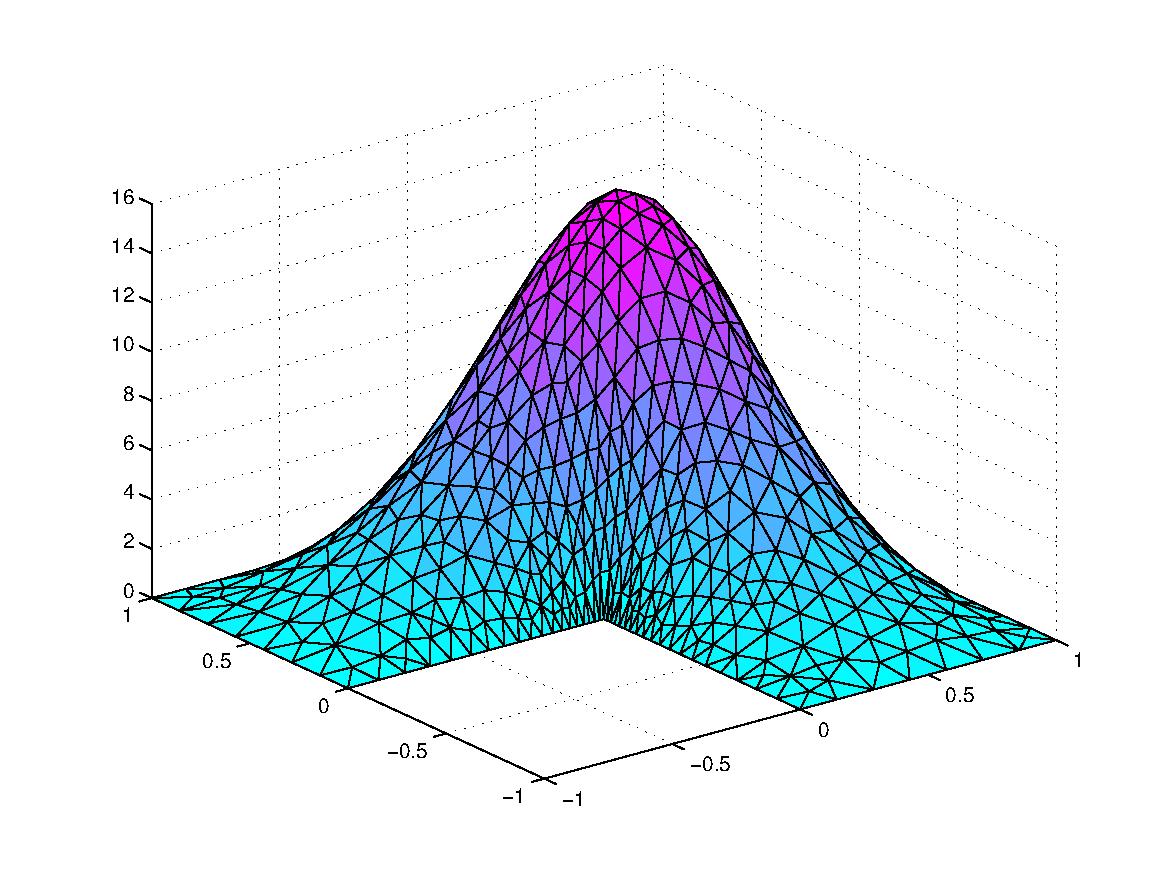
\includegraphics[width=100mm]{figure.pdf}
\caption{Include all graphics in the manuscript file.}
\label{fig:example}
\end{figure}

\subsection{Tables}
Tables are placed in the document in the same manner as figures.
Tables are referred to as Table~\ref{tab:example}.
Table captions are placed above the corresponding tables.

\begin{table}[htb]
\caption{Table example}
\centering
\begin{tabular}{
  c||
  S[table-format=1.2e-1]
  S[table-format=1.2]
  S[table-format=1.2e-1]
  S[table-format=1.2]
  S[table-format=1.2e-1]
  S[table-format=1.2]
  S[table-format=1.2e-1]
  S[table-format=1.2]
}
\hline
\multicolumn{1}{c||}{$h$} & \mcc{$M_{h,1}$} & \mcc{order} &
\mcc{$M_{h,1}(f)$} & \mcc{order} & \mcc{$M_{h,2}$} &
\mcc{order} & \mcc{$M_{h,2}(f)$} & \mcc{order} \\
\hline
1/2 & 2.61e-1 & \mcc{-} & 1.81e-1 & \mcc{-} & 1.90e-1 & \mcc{-} & 4.19e-2 & \mcc{-} \\
1/4 & 1.37e-1 & 0.93 & 9.8e-2 & 0.89 & 9.63e-2 & 0.98 & 1.26e-2 & 1.73 \\
1/8 & 7.08e-2 & 0.95 & 5.0e-2 & 0.96 & 4.84e-2 & 0.99 & 3.60e-3 & 1.81 \\
1/16 & 3.65e-3 & 0.96 & 2.5e-2 & 0.99 & 2.43e-2 & 1.00 & 9.96e-4 & 1.85 \\
1/32 & 1.85e-4 & 0.98 & 1.3e-2 & 1.00 & 1.21e-2 & 1.00 & 2.72e-4 & 1.88 \\
\hline
\end{tabular}
\label{tab:example}
\end{table}%

%%%%%%%%%%%%%%%%%%%
% Acknowledgement
%%%%%%%%%%%%%%%%%%%
\acknowledgement
Acknowledgements, if any, can be placed just after the last section (usually just after ``Conclusions'').
Your acknowledgements to co-workers and financial sponsors are placed here.

%%%%%%%%%%%%%%%%%%%
% Appendices
%%%%%%%%%%%%%%%%%%%
\appendix
\section{Style of an appendix}
Appendices, if any, can be placed after the Acknowledgements, but before the References. Appendix headings are numbered in alphabet order (like A, B, C).

\section{Second appendix}
This is a second appendix of the paper.

%%%%%%%%%%%%%%%%%%%
% References
%%%%%%%%%%%%%%%%%%%
\nocite{journal_paper,journal_paper_example,inproceedings,inproceedings_example,book,book_example,book_chapter,book_chapter_example,arxiv,arxiv_example,webpage,webpage_example}
\bibliographystyle{jasse}
\bibliography{JSST2026_refs}

\end{document}
